\documentclass[12pt,a4paper]{article}

% ── Encodage & langue ─────────────────────────────────────
\usepackage[utf8]{inputenc}
\usepackage[T1]{fontenc}
\usepackage[english]{babel}

% ── Mise en page ──────────────────────────────────────────
\usepackage[top=2.5cm,bottom=2.5cm,left=3cm,right=3cm]{geometry}
\usepackage{setspace}
\onehalfspacing

% ── Mathématiques ─────────────────────────────────────────
\usepackage{amsmath,amssymb,amsthm}
\usepackage{mathtools}

% ── Graphiques & couleurs ─────────────────────────────────
\usepackage{graphicx}
\usepackage[dvipsnames,svgnames,x11names]{xcolor}
\usepackage{tikz}
\usetikzlibrary{arrows.meta,positioning,shapes,fit,backgrounds}

% ── Tableaux ──────────────────────────────────────────────
\usepackage{booktabs}
\usepackage{array}
\usepackage{multirow}

% ── Liens & métadonnées ───────────────────────────────────
\usepackage{hyperref}
\hypersetup{
  colorlinks=true,
  linkcolor=NavyBlue,
  citecolor=NavyBlue,
  urlcolor=NavyBlue,
  pdftitle={CommunityTrust Protocol},
  pdfauthor={OpenScience Community},
}

% ── Algorithmes ───────────────────────────────────────────
\usepackage{algorithm}
\usepackage{algpseudocode}

% ── En-têtes ──────────────────────────────────────────────
\usepackage{fancyhdr}
\pagestyle{fancy}
\fancyhf{}
\rhead{\small\textcolor{gray}{CTP v1.1 --- OpenScience Community}}
\lhead{\small\textcolor{gray}{CommunityTrust Protocol}}
\cfoot{\thepage}

% ── Environnements théoriques ─────────────────────────────
\theoremstyle{definition}
\newtheorem{definition}{Définition}[section]
\newtheorem{exemple}{Exemple}[section]

\theoremstyle{plain}
\newtheorem{theoreme}{Théorème}[section]
\newtheorem{proposition}{Proposition}[section]
\newtheorem{lemme}{Lemme}[section]
\newtheorem{corollaire}{Corollaire}[section]

\theoremstyle{remark}
\newtheorem{remarque}{Remarque}[section]

% ── Commandes personnalisées ──────────────────────────────
\newcommand{\CTP}{\textsc{ctp}}
\newcommand{\trustscore}{\tau}
\newcommand{\R}{\mathbb{R}}
\newcommand{\N}{\mathbb{N}}
\newcommand{\E}{\mathbb{E}}
\newcommand{\1}{\mathbf{1}}
\newcommand{\clip}{\operatorname{clip}}

% ─────────────────────────────────────────────────────────
\begin{document}

% ── Page de titre ─────────────────────────────────────────
\begin{titlepage}
\centering
\vspace*{1.5cm}

{\Large \textsc{OpenScience Community}}\\[0.4cm]
{\small Protocole Technique — Document de Référence}\\[2cm]

\hrule height 0.5pt
\vspace{0.6cm}

{\Huge \textbf{CommunityTrust Protocol}}\\[0.5cm]
{\LARGE \textit{CTP v1.1}}\\[0.3cm]

\vspace{0.4cm}
\hrule height 0.5pt
\vspace{1.2cm}

{\large \textit{``Je suis parce que nous sommes''}}\\[0.2cm]
{\small \textit{--- Ubuntu Philosophy, Southern Africa}}

\vspace{1.5cm}

{\large A universal community trust protocol\\
inspired by African tontines,\\
formalized through mathematics,\\
validated by simulation,\\
designed for smart contracts.}

\vspace{1.5cm}

\begin{tabular}{rl}
\textbf{Author}       & Ange AWALA \\
\textbf{Affiliation}  & OpenScience Community \\
\textbf{Contact}      & openscience.community@proton.me \\[0.3cm]
\textbf{Version}      & 1.1 --- Corrections and Extensions \\
\textbf{Status}       & Open Research \\
\textbf{License}      & Creative Commons BY-SA 4.0 \\
\textbf{Repository}   & Zenodo --- DOI: 10.5281/zenodo.20031237 \\
\end{tabular}

\vfill
{\small \today}
\end{titlepage}

% ── Résumé ────────────────────────────────────────────────
\begin{abstract}
\noindent
Existing trust systems measure popularity, wealth, or
institutional status. The \textbf{CommunityTrust Protocol} (\CTP{}) proposes
a radical alternative: measuring \emph{behavioral reliability over
time}, independently of any pre-existing financial or social capital.

Inspired by the logic of African tontines---decentralized community financing
systems where collective trust replaces bank
guarantees---\CTP{} formalizes a universal reputation engine applicable to
any community-based system: social networks, decentralized autonomous
organizations (DAOs), knowledge cooperatives, and
micro-finance systems.

This document presents: (1) the complete conceptual specification of the
protocol, (2) a rigorous mathematical model including the
\emph{TrustScore} dynamics, the \emph{Witness} accountability mechanism, and the
\emph{Node} hierarchy, (3) a game-theoretic analysis
guaranteeing resistance to strategic behaviors, and (4) empirical
validation through Monte Carlo simulation over 52 periods.

Results demonstrate that honest behaviors strictly dominate
free-riding, collusion, and desertion strategies under the
recommended parameters. All three theoretical propositions are empirically verified.

\medskip\noindent
\textbf{New in v1.1:} (a) Capital of Forgiveness --- adaptive gain rate
$\eta_i(t)$ based on seniority; (b) directional semantic similarity
$\operatorname{sim}(j \to j')$ calculable on-chain~; (c) analyse de
complexity analysis and gas costs; (d) foundational reference Marsh
(1994) formally positioned; (e) explicit limitations section; (f) correction of
parameter $\rho_r$ in the Finance module.

\medskip
\noindent\textbf{Keywords:} community trust, tontine, decentralized
reputation, game theory, smart contracts, open science, P2P
protocol.
\end{abstract}

\newpage
\tableofcontents
\newpage

% ═════════════════════════════════════════════════════════
\section{Introduction}
% ═════════════════════════════════════════════════════════

\subsection{Motivation}

Les communautés humaines ont développé depuis des millénaires des mécanismes
sophistiqués de confiance collective sans recours aux institutions financières
formelles. La \textbf{tontine} --- pratique répandue à travers l'Afrique,
l'Asie et la diaspora africaine mondiale --- en constitue l'exemple le plus
remarquable~: un groupe de personnes contribue périodiquement à un pot commun,
redistribué à tour de rôle selon des règles négociées collectivement. Ce
système fonctionne sans contrat légal, sans garantie bancaire, uniquement sur
la base de la réputation et de la pression sociale.

Ce qui rend les tontines efficaces n'est pas l'argent en jeu, mais
l'\textbf{information communautaire}~: chaque membre connaît le comportement
passé de ses pairs, et cette connaissance structure les incitations présentes
et futures. La confiance est une ressource circulante, construite lentement et
perdue rapidement.

Les systèmes numériques contemporains ont largement échoué à capturer cette
logique. Les réseaux sociaux mesurent la popularité algorithmique. Les DAOs
confondent richesse et gouvernance. Les plateformes de micro-finance importent
des modèles bancaires inadaptés aux contextes de faible bancarisation. Aucun
ne formalise ce que les tontines font naturellement~: \emph{quantifier la
fiabilité relationnelle dans le temps}.

\subsection{Contributions}

Le \textbf{CommunityTrust Protocol} (\CTP{}) apporte les contributions
suivantes~:

\begin{enumerate}
  \item \textbf{Universalité}~: un moteur de réputation unique applicable à
    tout système communautaire, paramétrable sans modification du code central.

  \item \textbf{Ancrage théorique}~: une formalisation mathématique rigoureuse
    des mécanismes de confiance communautaire africaine, jusqu'ici transmis
    oralement.

  \item \textbf{Résistance stratégique}~: une analyse par la théorie des jeux
    prouvant que les comportements honnêtes constituent un équilibre dominant
    sous les paramètres recommandés.

  \item \textbf{Implémentabilité}~: une architecture directement traduisible
    en smart contracts, conçue dès l'origine pour l'exécution décentralisée.

  \item \textbf{Hiérarchie de Nodes}~: un système multi-niveaux
    (Meta-Node~/ Node~/ Sub-Node) permettant la coexistence de communautés
    autonomes partageant un socle commun de règles éthiques.
\end{enumerate}

\subsection{Document Structure}

La Section~\ref{sec:concepts} introduit le vocabulaire fondateur. La
Section~\ref{sec:modele} présente le modèle mathématique complet. La
Section~\ref{sec:jeux} analyse les équilibres stratégiques. La
Section~\ref{sec:simulation} valide les résultats par simulation. La
Section~\ref{sec:architecture} décrit l'architecture des Nodes. La
Section~\ref{sec:ethique} pose les principes éthiques fondateurs. La
Section~\ref{sec:conclusion} conclut et ouvre les perspectives.

% ═════════════════════════════════════════════════════════
\section{Conceptual Specification}
\label{sec:concepts}
% ═════════════════════════════════════════════════════════

\subsection{Founding Vocabulary}

\CTP{} repose sur cinq concepts primitifs dont les définitions sont
immuables~: aucune implémentation ne peut les redéfinir.

\begin{definition}[Signal]
Un \textbf{Signal} $s$ est tout acte brut produit librement par un membre~:
publication, paiement, vote, partage de ressource. Le Signal n'a pas de valeur
a priori --- il existe simplement comme événement observable.
\end{definition}

\begin{definition}[Contribution]
Une \textbf{Contribution} est un Signal validé collectivement par un nombre
suffisant de Witnesses. C'est l'unité de base du protocole. Sans validation
communautaire, il n'existe pas de Contribution.
\end{definition}

\begin{definition}[Witness]
Un \textbf{Witness} est un membre dont le TrustScore dépasse un seuil fixé par
le Node, habilité à valider des Signals. Le Witness engage sa propre réputation
dans l'acte de validation~: valider un Signal de mauvaise qualité a un coût.
\end{definition}

\begin{definition}[TrustScore]
Le \textbf{TrustScore} $\trustscore_{i,j}(t) \in [0,1]$ est le score de
réputation du membre $i$ dans le Node $j$ au temps $t$. Il ne se vend pas, ne
se transfère pas et ne s'achète pas. Il se construit uniquement par le
comportement observé dans le temps.
\end{definition}

\begin{definition}[Node]
Un \textbf{Node} $N_j$ est une communauté qui implémente \CTP{}. Il définit
ses propres paramètres de validation dans les limites fixées par le Meta-Node.
Des exemples de Nodes~: une tontine de quartier, un groupe de recherche
scientifique, une coopérative agricole, une DAO.
\end{definition}

\subsection{Cycle de vie d'une Contribution}

Le cycle de vie complet d'un Signal est représenté à la
Figure~\ref{fig:cycle}.

\begin{figure}[h]
\centering
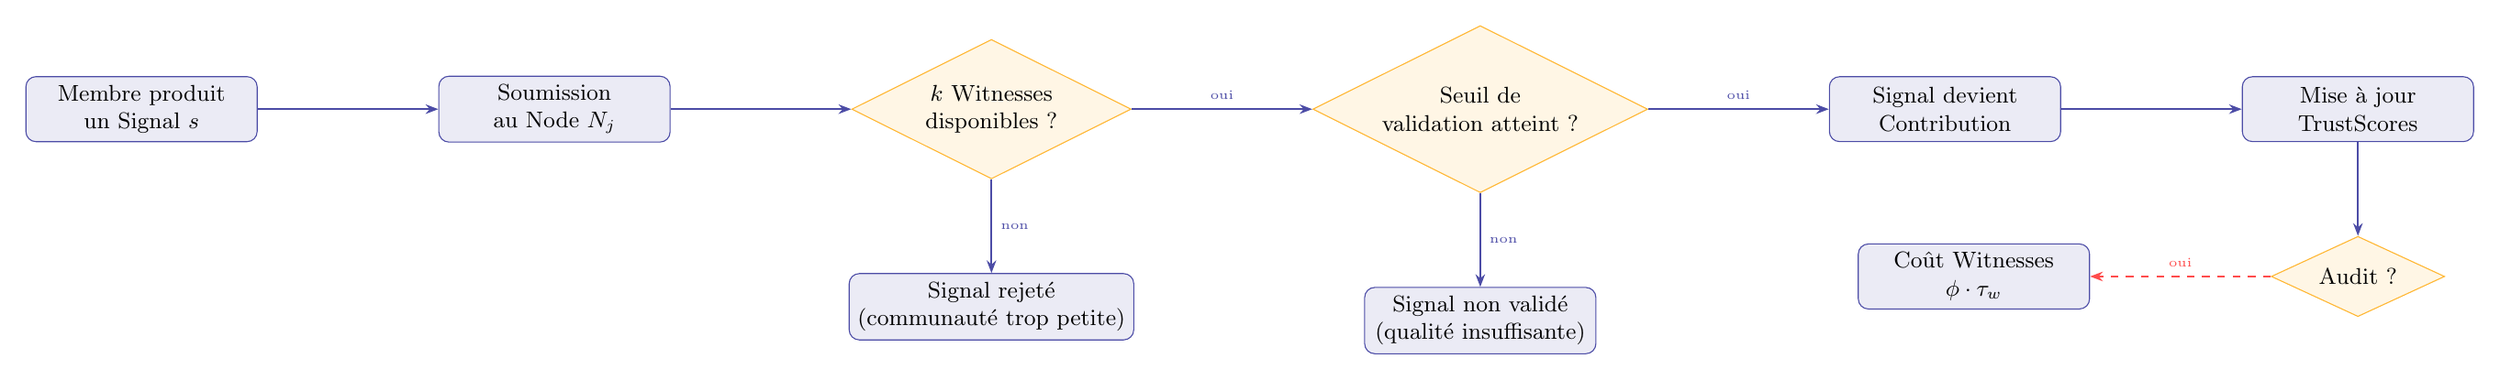
\begin{tikzpicture}[
  node distance=1.3cm and 2.5cm,
  box/.style={rectangle,rounded corners=4pt,draw=NavyBlue!70,
              fill=NavyBlue!8,minimum width=3.2cm,minimum height=0.9cm,
              font=\small,align=center},
  decision/.style={diamond,draw=Orange!80,fill=Orange!10,
                   minimum width=2.4cm,minimum height=0.9cm,
                   font=\small,align=center,aspect=2},
  arr/.style={-{Stealth[length=5pt]},NavyBlue!70,thick},
  warn/.style={-{Stealth[length=5pt]},Red!70,thick,dashed},
]

\node[box] (prod) {Membre produit\\un Signal $s$};
\node[box,right=of prod] (soum) {Soumission\\au Node $N_j$};
\node[decision,right=of soum] (wit) {$k$ Witnesses\\disponibles~?};
\node[box,below=of wit] (rej1) {Signal rejeté\\(communauté trop petite)};
\node[decision,right=of wit] (val) {Seuil de\\validation atteint~?};
\node[box,below=of val] (rej2) {Signal non validé\\(qualité insuffisante)};
\node[box,right=of val] (contrib) {Signal devient\\Contribution};
\node[box,right=of contrib] (update) {Mise à jour\\TrustScores};
\node[decision,below=of update] (audit) {Audit~?};
\node[box,left=of audit] (cout) {Coût Witnesses\\$\phi\cdot\trustscore_w$};

\draw[arr] (prod)    -- (soum);
\draw[arr] (soum)    -- (wit);
\draw[arr] (wit)     -- node[right,font=\tiny]{non} (rej1);
\draw[arr] (wit)     -- node[above,font=\tiny]{oui} (val);
\draw[arr] (val)     -- node[right,font=\tiny]{non} (rej2);
\draw[arr] (val)     -- node[above,font=\tiny]{oui} (contrib);
\draw[arr] (contrib) -- (update);
\draw[arr] (update)  -- (audit);
\draw[warn](audit)   -- node[above,font=\tiny]{oui} (cout);

\end{tikzpicture}
\caption{Cycle de vie d'un Signal dans \CTP{}.}
\label{fig:cycle}
\end{figure}

\subsection{Founding Principle}

Le principe central de \CTP{} peut s'énoncer ainsi~:

\begin{center}
\fbox{\parbox{0.85\textwidth}{\centering\itshape
La confiance d'un membre est la somme de ses comportements observés,\\
pondérée par la fiabilité de ceux qui les ont observés.
}}
\end{center}

Ce principe implique une récursivité constitutive~: la valeur d'une validation
dépend de la réputation du validateur, qui elle-même dépend de ses validations
passées. Cela crée une structure d'incitations auto-renforçante favorable aux
comportements honnêtes.

% ═════════════════════════════════════════════════════════
\section{Mathematical Model}
\label{sec:modele}
% ═════════════════════════════════════════════════════════

\subsection{Spaces and Notation}

Soit un Meta-Node $\mathcal{M}$ contenant $m$ Nodes $\mathcal{N} = \{N_1,
\ldots, N_m\}$. Chaque Node $N_j$ contient un ensemble de membres
$\mathcal{M}_j = \{1, \ldots, n_j\}$. Le système évolue en périodes discrètes
$t \in \N$, dont la durée (hebdomadaire, mensuelle) est définie par chaque
Node.

\subsection{TrustScore Dynamics}

\subsubsection{Équation d'évolution}

Le TrustScore du membre $i$ dans le Node $j$ évolue selon~:

\begin{equation}
\boxed{
\trustscore_{i,j}(t+1) = \clip\!\Bigl(
  \trustscore_{i,j}(t) + G_{i,j}(t) - L_{i,j}(t) - D_{i,j}(t) - W_{i,j}(t),\;
  0,\; 1
\Bigr)
}
\label{eq:trust}
\end{equation}

où $\clip(x, 0, 1) = \max(0, \min(1, x))$ garantit la bornitude dans $[0,1]$.

\subsubsection{Force 1 --- Contribution Gain}

\begin{equation}
G_{i,j}(t) = \eta \sum_{k=1}^{K_{i,j}(t)} q(s_k)
\label{eq:gain}
\end{equation}

où $\eta \in (0,1)$ est le taux d'apprentissage du Node (petit, car la
confiance se construit lentement), $K_{i,j}(t)$ est le nombre de Contributions
validées à la période $t$, et $q(s_k) \in [0,1]$ est la qualité de la
$k$-ième Contribution définie à l'équation~\eqref{eq:quality}.

\subsubsection{Force 2 --- Default Penalty}

\begin{equation}
L_{i,j}(t) = \kappa \cdot \1_{\{\text{défaut}_i\}}(t)
\label{eq:loss}
\end{equation}

où $\kappa \in (0,1)$ est la pénalité de défaut, avec la contrainte
$\kappa \gg \eta$~: on perd rapidement ce que l'on a construit lentement,
conformément à la dynamique réelle de la confiance humaine.

\subsubsection{Force 3 --- Inactivity Depreciation}

\begin{equation}
D_{i,j}(t) = \delta \cdot \trustscore_{i,j}(t) \cdot \1_{\{\text{inactif}_i\}}(t)
\label{eq:depreciation}
\end{equation}

où $\delta \in (0,1)$ est le taux de dépréciation. La dépréciation est
proportionnelle au score courant~: les membres établis ont davantage à perdre
en restant inactifs. Ce mécanisme empêche de vivre sur ses acquis.

\subsubsection{Extension v1.1 --- Capital of Forgiveness}

Un défaut accidentel d'un membre de longue date ne doit pas être traité
de façon identique à une fraude d'un nouveau venu. \CTP{} v1.1 introduit
an \textbf{adaptive gain rate}:

\begin{equation}
\boxed{\eta_i(t) = \eta \cdot \left(1 + \alpha_P \cdot
\frac{h_{i,j}(t)}{T_{\text{ref}}}\right)}
\label{eq:pardon}
\end{equation}

where $\alpha_P \in [0,1]$ is the forgiveness amplifier and
$T_{\text{ref}}$ is a reference period (recommended value:
52 periods). A member active for two years ($h = 104$) rebuilds
son score environ deux fois plus vite qu'un nouveau venu après un défaut.

\begin{remarque}
The Capital of Forgiveness does not reduce the penalty $\kappa$ --- the fall
remains equally brutal for everyone. Only the \emph{speed of
reconstruction} est modulée par l'ancienneté. L'équité de la punition
est préservée~; la reconnaissance de l'historique ne l'est pas.
\end{remarque}

\begin{proposition}[Convergence with Capital of Forgiveness]
Under constant behavior and active Capital of Forgiveness, the TrustScore
of a long-standing member converges to:
$$\trustscore_i^* = \frac{\eta_i \cdot \bar{q}}{\eta_i \cdot \bar{q} + \epsilon}$$
which is strictly greater than $\trustscore^*$ without Capital of Forgiveness,
all else being equal.
\end{proposition}

\subsubsection{Force 4 --- Poor Validation Cost}

\begin{equation}
W_{i,j}(t) = \phi \sum_{s \,:\, i \in \mathcal{W}(s),\; s \text{ audité}}
\frac{\trustscore_{i,j}(t)}{|\mathcal{W}(s)|}
\label{eq:witness_cost}
\end{equation}

où $\phi \in (0,1)$ est le coefficient de responsabilité et $\mathcal{W}(s)$
l'ensemble des Witnesses du Signal $s$. Ce terme est la contribution centrale
de \CTP{} par rapport aux systèmes existants~: valider un Signal de mauvaise
qualité a un coût réel, partagé entre les Witnesses et proportionnel à leur
réputation.

\subsection{Qualité d'une Contribution}

La qualité d'un Signal validé est~:

\begin{equation}
q(s) = \bar{\trustscore}_{\mathcal{W}(s)} \cdot \rho(s)
= \frac{\sum_{w \in \mathcal{W}(s)} \trustscore_{w,j}(t)}{|\mathcal{W}(s)|}
\cdot \min\!\left(\frac{|\mathcal{W}(s)|}{k_j},\, 1\right)
\label{eq:quality}
\end{equation}

où $k_j$ est le seuil minimal de Witnesses du Node $j$, et $\rho(s) \in [0,1]$
est le taux de consensus. Une Contribution validée à l'unanimité par des
membres expérimentés vaut davantage qu'une Contribution validée de justesse par
des débutants.

\subsection{Adaptive Witness Threshold}

Pour éviter le blocage dans les petites communautés, le seuil de validation est
adaptatif~:

\begin{equation}
k_j = \max\!\left(k_{\min},\, \left\lfloor \alpha_k \cdot |\mathcal{M}_j| \right\rfloor\right)
\label{eq:k}
\end{equation}

avec $k_{\min} = 3$ et $\alpha_k = 0{,}20$ (valeurs recommandées par le
Meta-Node). Un Node de 20 membres requiert $\max(3, 4) = 4$ Witnesses~; un
Node de 5 membres requiert $\max(3, 1) = 3$ Witnesses.

\subsection{Global TrustScore and Node Hierarchy}

\subsubsection{Global Score in the Meta-Node}

Un membre appartenant à $m'$ Nodes simultanément possède un TrustScore Global~:

\begin{equation}
\trustscore_i^{\mathcal{M}}(t)
= \sum_{j=1}^{m'} \omega_{i,j}(t) \cdot \trustscore_{i,j}(t)
\label{eq:global}
\end{equation}

avec les poids~:

\begin{equation}
\omega_{i,j}(t) = \frac{h_{i,j}(t) \cdot \rho_j}{\displaystyle\sum_{j'=1}^{m'} h_{i,j'}(t) \cdot \rho_{j'}}
\label{eq:omega}
\end{equation}

où $h_{i,j}(t)$ est le nombre de périodes actives du membre $i$ dans le Node
$j$, et $\rho_j$ est l'indice de difficulté du Node défini ci-dessous.

\subsubsection{Indice de difficulté d'un Node}

\begin{equation}
\rho_j = \frac{k_j \cdot \bar{\trustscore}_j}{k_{\min} \cdot \trustscore_{\min}}
\label{eq:difficulty}
\end{equation}

où $\bar{\trustscore}_j$ est le TrustScore moyen des membres actifs du Node
$j$, et $\trustscore_{\min}$ est la valeur minimale observée sur l'ensemble du
Meta-Node. \textbf{L'indice de difficulté n'est jamais déclaré par le Node
lui-même~: il est calculé automatiquement à partir de données observables.}

\subsubsection{Inter-Node Portability}

Lorsqu'un membre $i$ rejoint un nouveau Node $j'$ sans historique, son score
initial est~:

\begin{equation}
\trustscore_{i,j'}(0) = \lambda_{\text{eff}}(m_i) \cdot \trustscore_i^{\mathcal{M}}(t)
\label{eq:portability}
\end{equation}

avec le coefficient de portabilité effectif~:

\begin{equation}
\lambda_{\text{eff}}(m_i) = \lambda \cdot \mu^{m_i} \cdot \operatorname{sim}(j_{\text{origine}}, j')
\label{eq:lambda_eff}
\end{equation}

où $m_i$ est le nombre de migrations récentes du membre, $\mu \in (0,1)$ est
la pénalité de migration fréquente, et $\operatorname{sim}(j, j') \in [0,1]$
est la similarité sémantique entre les deux Nodes, définie par le Meta-Node.
Le Node d'accueil peut abaisser $\lambda$ en-deçà de cette valeur, jamais
l'augmenter.

\paragraph{Extension v1.1 --- Similarité directionnelle basée sur les flux.}

En v0.1, $\operatorname{sim}(j, j')$ était spécifiée sans être calculable.
\CTP{} v1.1 proposes a direct, on-chain formalization based on
real member behaviors:

\begin{equation}
\boxed{\operatorname{sim}(j \to j') =
\frac{|\mathcal{M}_j \cap \mathcal{M}_{j'}|}{|\mathcal{M}_j|}}
\label{eq:sim}
\end{equation}

This is the proportion of members of Node $j$ who also belong to
Node $j'$. Cette mesure est~:

\begin{itemize}
  \item \textbf{Directionnelle}~: $\operatorname{sim}(j \to j') \neq
    \operatorname{sim}(j' \to j)$ en général. Si beaucoup de
    mathematicians join the Physics Node but few physicists
    rejoignent Mathématiques, la similarité n'est pas symétrique.
  \item \textbf{On-chain computable}: the sets $\mathcal{M}_j$
    et $\mathcal{M}_{j'}$ sont disponibles directement dans CTPCore.
  \item \textbf{Self-correcting}: if migration habits
    change, $\operatorname{sim}$ changes automatically without
    human intervention.
  \item \textbf{Manipulation-resistant}: a single individual cannot
    significantly modify the similarity between two
    reasonably-sized Nodes.
\end{itemize}

\begin{proposition}[Boundedness of sim]
$\operatorname{sim}(j \to j') \in [0,1]$ pour tout $j, j'$, avec
$\operatorname{sim}(j \to j) = 1$ et
$\operatorname{sim}(j \to j') = 0$ si $\mathcal{M}_j \cap \mathcal{M}_{j'} = \emptyset$.
\end{proposition}

\subsection{Voting Power}

Le droit de décision du membre $i$ dans le Node $j$ est~:

\begin{equation}
V_{i,j}(t) = \frac{\trustscore_{i,j}(t)}{\displaystyle\sum_{k \in \mathcal{M}_j} \trustscore_{k,j}(t)}
\label{eq:vote}
\end{equation}

Le vote est proportionnel au TrustScore, non à la richesse ni à l'ancienneté brute.

\subsection{Formal Properties}

\begin{proposition}[Bornitude]
Pour tout membre $i$, Node $j$ et temps $t \geq 0$~:
$$\trustscore_{i,j}(t) \in [0, 1]$$
\end{proposition}

\begin{proof}
Par initialisation $\trustscore_{i,j}(0) \in [0,1]$. La fonction $\clip$ dans
l'équation~\eqref{eq:trust} garantit que la propriété est préservée à chaque
étape par induction.
\end{proof}

\begin{proposition}[Convergence sous comportement constant]
Si un membre contribue régulièrement avec qualité moyenne $\bar{q}$, sans
défaut ($p_i = 0$) et sans inactivité ($a_i = 1$), son TrustScore converge
vers~:
$$\trustscore_i^* = \frac{\eta \cdot \bar{q}}{\eta \cdot \bar{q} + \epsilon}$$
où $\epsilon \to 0$ lorsque $\phi \to 0$. En pratique, $\trustscore_i^*$ tend
vers $1$ pour un membre parfaitement fiable.
\end{proposition}

\begin{proposition}[Résistance à l'accumulation passive]
Un membre inactif voit son TrustScore décroître géométriquement~:
$$\trustscore_{i,j}(t) = \trustscore_{i,j}(0) \cdot (1-\delta)^t \xrightarrow{t \to \infty} 0$$
Aucun membre ne peut maintenir un score élevé sans contribution active.
\end{proposition}

% ═════════════════════════════════════════════════════════
\section{Game Theory Analysis}
\label{sec:jeux}
% ═════════════════════════════════════════════════════════

\subsection{General Framework}

Chaque membre $i$ est modélisé comme un joueur rationnel maximisant son
utilité espérée sur un horizon $T$~:

\begin{equation}
U_i = \E\left[\sum_{t=0}^{T} \beta^t \cdot u_i(t)\right]
\label{eq:utility}
\end{equation}

où $\beta \in (0,1)$ est le facteur d'escompte temporel --- un membre
\og{}myope\fg{} a $\beta \approx 0$, un membre avec vision à long terme a
$\beta \approx 1$ --- et l'utilité instantanée est~:

\begin{equation}
u_i(t) = f(\trustscore_{i,j}(t)) - c_i(t)
\end{equation}

où $f : [0,1] \to \R_+$ est une fonction croissante représentant les droits
conférés par le TrustScore (accès aux ressources, pouvoir de vote, financement)
et $c_i(t)$ est le coût réel de la contribution à la période $t$.

\subsection{Game 1 --- The Free Rider}

\subsubsection{Formalisation}

Le membre $i$ choisit entre contribuer (stratégie $C$, coût $c > 0$) ou
parasiter (stratégie $P$, coût nul). Sous stratégie $P$, le score décroît
par la dépréciation~: $\trustscore_i(t) = \trustscore_i(0)(1-\delta)^t$.

\subsubsection{Condition de dominance}

La stratégie $C$ domine $P$ si et seulement si~:

\begin{equation}
\sum_{t=0}^{T} \beta^t \left[f(\trustscore_i^C(t)) - f\!\left(\trustscore_i(0)(1-\delta)^t\right)\right] > c \cdot T
\label{eq:freerider}
\end{equation}

\begin{proposition}[Neutralisation du free-riding]
Si $f(\trustscore)$ est suffisamment croissante --- c'est-à-dire si les droits
associés au TrustScore ont une valeur réelle --- et si $\beta$ est
suffisamment proche de 1, alors la stratégie $C$ domine strictement $P$.
\end{proposition}

\begin{remarque}
\textbf{Implication critique pour l'implémentation~:} les droits associés au
TrustScore ne sont pas optionnels. Un Node qui n'attache aucun droit réel au
score crée mécaniquement du free-riding. La valeur de $f$ est le premier levier
de conception.
\end{remarque}

\subsection{Game 2 --- Witness Collusion}

\subsubsection{Formalisation}

Ce jeu est modélisé comme un \textbf{dilemme du prisonnier répété} entre un
membre $i$ et ses Witnesses complices potentiels. À chaque période, chaque
Witness choisit entre valider honnêtement (H) ou colluder (K).

\subsubsection{Analyse des payoffs}

Pour un Witness $w$ participant à la collusion~:

\begin{align}
G_{\text{collusion}} &= \eta \cdot q_{\text{artificiel}} \cdot N_{\text{validés}} \\
C_{\text{détection}} &= \phi \cdot \trustscore_w(t) \cdot \mathbb{P}(\text{détection})
\end{align}

\begin{proposition}[Condition anti-collusion]
La collusion est irrationnelle pour le Witness si~:

\begin{equation}
\phi > \frac{\eta \cdot q_{\text{artificiel}}}{\trustscore_w(t) \cdot \mathbb{P}(\text{détection})}
\label{eq:anticollusion}
\end{equation}

En particulier, la condition $\phi \geq 3\eta$ est suffisante pour
$\trustscore_w \geq 0{,}3$ et $\mathbb{P}(\text{détection}) \geq 0{,}15$.
\end{proposition}

\subsubsection{Équilibre dans le jeu répété}

Dans un jeu répété à horizon infini avec $\beta$ suffisamment grand, la
stratégie \textit{Tit-for-Tat honnête} --- être honnête, punir immédiatement
toute collusion détectée, reprendre la coopération si le comportement redevient
honnête --- constitue un équilibre de Nash sous~:

\begin{equation}
\beta > \frac{\phi \cdot \trustscore_w \cdot \mathbb{P}(\text{détection})}{\eta \cdot q_{\text{artificiel}}}
\label{eq:tft}
\end{equation}

\subsection{Game 3 --- Strategic Deserter}

\subsubsection{Formalisation}

Le déserteur entre dans un Node, monte son score minimalement, extrait les
droits disponibles, puis migre vers un nouveau Node en emportant sa
portabilité. Son utilité sur $m$ migrations est~:

\begin{equation}
U_{\text{déserteur}} = \sum_{j=1}^{m} \left[f(\lambda_{\text{eff}}(j) \cdot \trustscore^{\mathcal{M}}) - c_{\min} \cdot T_j\right]
\end{equation}

\subsubsection{Mécanismes de neutralisation}

Trois mécanismes combinés rendent cette stratégie irrationnelle~:

\begin{enumerate}
  \item \textbf{Dépréciation du score global~:} $\trustscore^{\mathcal{M}}(t) \to 0$ en l'absence de contribution réelle.
  \item \textbf{Pénalité de migration~:} $\lambda_{\text{eff}}(m) = \lambda \cdot \mu^m \cdot \operatorname{sim}(j, j')$ décroît exponentiellement avec $m$.
  \item \textbf{Distance sémantique~:} $\operatorname{sim}(j, j') \approx 0$ pour des domaines éloignés.
\end{enumerate}

\begin{proposition}[Neutralisation de la désertion]
Pour $\mu \in [0{,}6, 0{,}8]$ et $\beta$ suffisamment grand, la stratégie de
désertion est dominée par la contribution honnête dans un seul Node.
\end{proposition}

\subsection{Equilibrium Summary}

\begin{table}[h]
\centering
\caption{Résumé des conditions de résistance stratégique de \CTP{}.}
\label{tab:equilibres}
\begin{tabular}{llll}
\toprule
\textbf{Comportement} & \textbf{Mécanisme} & \textbf{Condition} & \textbf{Valeur rec.} \\
\midrule
Passager clandestin & Dépréciation $\delta$ + valeur de $f$ & $f$ croissante réelle & $\delta = 0{,}02$ \\
Collusion Witnesses & Responsabilité $\phi$ & $\phi \geq 3\eta$ & $\phi = 0{,}15$ \\
Déserteur & Pénalité $\mu$ + distance $\operatorname{sim}$ & $\mu \in [0{,}6, 0{,}8]$ & $\mu = 0{,}70$ \\
\bottomrule
\end{tabular}
\end{table}

% ═════════════════════════════════════════════════════════
\section{Simulation Validation}
\label{sec:simulation}
% ═════════════════════════════════════════════════════════

\subsection{Experimental Protocol}

La simulation est conduite sur un Node de 12 membres répartis en quatre
groupes comportementaux~: 5 membres honnêtes, 3 passagers clandestins, 2
colludeurs, 2 déserteurs. Le Node est simulé sur $T = 52$ périodes
(équivalent d'une année hebdomadaire). Les paramètres utilisés sont ceux du
Tableau~\ref{tab:parametres}.

\begin{table}[h]
\centering
\caption{Paramètres complets de \CTP{} v0.1.}
\label{tab:parametres}
\begin{tabular}{clll}
\toprule
\textbf{Paramètre} & \textbf{Rôle} & \textbf{Valeur} & \textbf{Contrainte} \\
\midrule
$\eta$   & Base gain rate                 & $0.05$    & $\eta \ll \kappa$ \\
$\alpha_P$ & Forgiveness amplifier        & $0.50$    & $\alpha_P \in [0,1]$ \\
$T_{\text{ref}}$ & Reference period        & $52$      & $T_{\text{ref}} > 0$ \\
$\kappa$ & Pénalité de défaut             & $0{,}15$  & $\kappa \gg \eta$ \\
$\delta$ & Dépréciation par inactivité    & $0{,}02$  & $\delta > 0$ \\
$\phi$   & Responsabilité Witness         & $0{,}15$  & $\phi \geq 3\eta$ \\
$\lambda$& Portabilité de base            & $0{,}20$  & $\lambda \in [0,1]$ \\
$\mu$    & Pénalité de migration          & $0{,}70$  & $\mu \in [0{,}6, 0{,}8]$ \\
$k_{\min}$ & Witnesses minimum            & $3$       & $k_{\min} \geq 3$ \\
$\alpha_k$ & Fraction adaptative          & $0{,}20$  & $\alpha_k \in (0,1)$ \\
\bottomrule
\end{tabular}
\end{table}

\subsection{Results}

Les résultats détaillés sont présentés à la Figure~\ref{fig:simulation}.

\begin{figure}[h]
\centering
\includegraphics[width=\textwidth]{ctp_analyse.png}
\caption{Résultats de simulation~: évolution des TrustScores sur 52 périodes,
scores finaux par comportement, analyse de sensibilité au paramètre $\delta$,
et vérification empirique des propositions théoriques. Les membres honnêtes
(vert) dominent strictement tous les autres comportements.}
\label{fig:simulation}
\end{figure}

\subsection{Proposition Verification}

Les trois propositions théoriques sont vérifiées empiriquement~:

\begin{enumerate}
  \item \textbf{Bornitude~:} $\trustscore_{i,j}(t) \in [0,1]$ pour tous les
    membres, toutes les périodes. \hfill \checkmark

  \item \textbf{Dominance honnête sur le free-riding~:}
    $\bar{\trustscore}_{\text{honnête}} = 1{,}000 \gg
    \bar{\trustscore}_{\text{passager}} = 0{,}104$. \hfill \checkmark

  \item \textbf{Dominance honnête sur la collusion~:}
    $\bar{\trustscore}_{\text{honnête}} = 1{,}000 \gg
    \bar{\trustscore}_{\text{colludeur}} = 0{,}292$. \hfill \checkmark
\end{enumerate}

\subsection{Sensitivity Analysis}

L'analyse de sensibilité au paramètre $\delta$ confirme que pour
$\delta \in [0{,}01, 0{,}05]$, l'écart entre membres honnêtes et passagers
clandestins reste significatif. La valeur $\delta = 0{,}02$ offre un bon
équilibre entre punition de l'inactivité et tolérance aux absences
occasionnelles.

% ═════════════════════════════════════════════════════════
\section{Architecture des Nodes}
\label{sec:architecture}
% ═════════════════════════════════════════════════════════

\subsection{Hiérarchie à trois niveaux}

\CTP{} organise les communautés selon une hiérarchie de contraintes
descendantes~:

\begin{description}
  \item[Meta-Node $\mathcal{M}$] Définit les règles éthiques minimales et la
    structure mathématique du protocole. Immuable pour toutes les
    implémentations. Calcule $\rho_j$ et $\operatorname{sim}(j, j')$.

  \item[Node $N_j$] Définit ses paramètres dans les limites du Meta-Node.
    Peut être plus strict, jamais plus lâche. Gère ses propres Witnesses et
    son propre cycle de validation.

  \item[Sub-Node $N_{j,k}$] Sous-communauté thématique d'un Node. Hérite des
    contraintes du Node parent et peut en ajouter.
\end{description}

Un membre peut appartenir simultanément à plusieurs Nodes~; son TrustScore
est local à chaque Node et contribue à son score global via
l'équation~\eqref{eq:global}.

\subsection{Gouvernance interne}

Les décisions structurelles d'un Node (modification des paramètres, exclusion
d'un membre, changement du seuil $k_j$) sont traitées comme des
\textbf{GovSignals}~: des Signals spéciaux soumis au même protocole de
validation mais avec des exigences renforcées~:

\begin{itemize}
  \item Seuil de Witnesses $k_{\text{gov}} \geq 2 k_j$
  \item TrustScore minimum des Witnesses dans le quartile supérieur du Node
  \item Délai de contestation d'une période complète
\end{itemize}

Si un GovSignal est contesté par un nombre suffisant de membres, il est
suspendu et soumis à un vote pondéré par TrustScore.

\subsection{Mécanisme d'audit}

Tout membre peut émettre un \textbf{ChallengeSignal} contre une Contribution
existante. Ce mécanisme est incitatif~:

\begin{itemize}
  \item \textbf{Coût du challenge~:} fraction $\phi_c \cdot \trustscore_i$
    du score du challenger --- pour éviter les contestations abusives.
  \item \textbf{Si le challenge est accepté~:} la Contribution est invalidée,
    les Witnesses originaux sont pénalisés via $\phi$, le challenger récupère
    sa mise plus un bonus.
  \item \textbf{Si le challenge est rejeté~:} le challenger perd sa mise, les
    Witnesses ne sont pas affectés.
\end{itemize}

% ═════════════════════════════════════════════════════════
\section{Principes Éthiques Fondateurs}
\label{sec:ethique}
% ═════════════════════════════════════════════════════════

\CTP{} est un protocole technique porteur d'une philosophie précise. Les
principes suivants ne sont pas des recommandations~: ils sont constitutifs du
protocole. Toute implémentation qui les viole n'est pas conforme à \CTP{}.

\begin{description}
  \item[Autonomie communautaire] \CTP{} renforce la capacité d'une communauté
    à se gouverner sans dépendre d'une institution extérieure. Il ne remplace
    pas l'État~; il rend la communauté moins dépendante de lui pour ses
    fonctions de coordination interne.

  \item[Réciprocité] Chaque membre contribue et reçoit. Le parasitisme à long
    terme est mécaniquement impossible sous les paramètres recommandés.

  \item[Mémoire courte réparable] Un défaut passé ne condamne pas à vie.
    Le TrustScore peut se reconstruire~; cela prend du temps, proportionnel à
    la gravité du manquement.

  \item[Transparence des règles, confidentialité des personnes] Les règles du
    Node sont publiques et auditables. Les scores individuels ne le sont que
    si le Node en décide collectivement.

  \item[Non-marchandisation du score] Le TrustScore n'est ni un token ni un
    actif financier. Il ne fluctue pas selon un marché. Il ne s'échange pas.
    Toute tentative de monétisation directe du score contredit la philosophie
    fondatrice du protocole.

  \item[Décentralisation des données] Chaque Node gère ses propres données.
    \CTP{} ne centralise rien. Le Meta-Node calcule $\rho_j$ et
    $\operatorname{sim}(j,j')$ à partir de données agrégées et anonymisées.
\end{description}

% ═════════════════════════════════════════════════════════
\section{Algorithmic Complexity and Implementation}
\label{sec:complexity}

\subsection{Complexity Analysis}

Table~\ref{tab:complexity} presents the complexity and estimated gas costs
on Polygon for each main function of the contract
\texttt{CTPCore.sol}.

\begin{table}[h]
\centering
\caption{Algorithmic complexity and estimated gas costs (Polygon mainnet).}
\label{tab:complexity}
\begin{tabular}{llll}
\toprule
\textbf{Function} & \textbf{Complexity} & \textbf{Estimated Gas} & \textbf{USD Cost} \\
\midrule
\texttt{createNode()}      & $O(1)$    & $\sim 120{,}000$     & $< 0{,}02$ \\
\texttt{joinNode()}        & $O(1)$    & $\sim 80{,}000$      & $< 0{,}01$ \\
\texttt{submitSignal()}    & $O(1)$    & $\sim 70{,}000$      & $< 0{,}01$ \\
\texttt{validateSignal()}  & $O(n)$    & $\sim 50{,}000 + 5{,}000n$ & Variable \\
\texttt{advancePeriod()}   & $O(n)$    & $\sim 20{,}000n$     & Variable \\
\texttt{auditSignal()}     & $O(n)$    & $\sim 30{,}000n$     & Variable \\
\texttt{getTrustScore()}   & $O(1)$    & Gratuit (lecture)    & $0$ \\
\bottomrule
\end{tabular}
\end{table}

\subsection{Batch Strategy for advancePeriod()}

The \texttt{advancePeriod()} function iterates over all Node members
--- $O(n)$ complexity. For large Nodes ($n > 50$),
gas may exceed the block limit. \CTP{} v1.1 recommends:

\begin{itemize}
  \item Processing batches of 50 members maximum:
    \texttt{advancePeriod(nodeId, 0, 50)}, \texttt{advancePeriod(nodeId, 50, 50)}, etc.
  \item La période n'avance qu'une fois tous les membres traités.
  \item Total cost: $\sim 20{,}000 \times n$ gas, i.e. $< 1.00$ USD
    for $n = 200$ members on Polygon.
\end{itemize}

\section{Related Work and Positioning}
\label{sec:related}
% ═════════════════════════════════════════════════════════

\subsection{Computational Trust --- Marsh (1994)}

The first mathematical formalization of computational trust is
due to Marsh~\cite{marsh1994trust}, whose 1994 thesis introduces
the concept of trust as a continuous variable between 0 and 1, with
propriétés de mise à jour basées sur l'expérience. \CTP{} étend ce cadre
framework by introducing: (1) collective community validation via
les Witnesses, (2) la hiérarchie de Nodes, et (3) l'ancrage dans la
Ubuntu philosophy and the logic of African tontines.

\subsection{Peer-to-Peer Reputation Systems}

Les travaux fondateurs sur EigenTrust~\cite{kamvar2003eigentrust}
et PeerTrust~\cite{xiong2004peertrust} mesurent la fiabilité
des nœuds dans des réseaux P2P à partir de l'historique des transactions.
\CTP{} s'en distingue sur trois points~: (1) l'introduction d'une
hiérarchie de Nodes paramétrable, (2) le mécanisme de responsabilité des
Witnesses qui engage la réputation du validateur, et (3) l'ancrage dans une
philosophie de confiance communautaire africaine plutôt que dans un modèle
purement transactionnel.

\subsection{Decentralized Governance and DAOs}

Les organisations autonomes décentralisées (DAOs) confondent généralement
richesse et gouvernance~: le pouvoir de vote est proportionnel au nombre de
tokens détenus. \CTP{} propose une alternative radicale où le pouvoir de vote
est proportionnel au TrustScore --- une mesure comportementale non monétisable.
Cette approche rejoint les préoccupations soulevées par Buterin sur les
limites des systèmes de gouvernance token-pondérés~\cite{buterin2021governance}.

\subsection{Formal Negotiation Modeling in Data Spaces}

Le travail récent de Daoudi, Lefrançois et Zimmermann~\cite{daoudi2026negotiation}
propose un cadre formel pour la négociation automatisée des contrats d'accès
aux données dans les espaces de données décentralisés. Leur approche identifie
explicitement l'absence d'un mécanisme garantissant la fiabilité des acteurs
au-delà de la négociation elle-même comme un verrou scientifique majeur.

\CTP{} répond précisément à ce manque~: le TrustScore fournit une mesure
continue de la fiabilité comportementale, le mécanisme de Witnesses assure
un audit communautaire continu des engagements, et la théorie des jeux
garantit la résistance aux comportements stratégiques post-contractuels.

Inversement, \CTP{} spécifie une fonction de similarité sémantique
$\operatorname{sim}(j, j')$ entre Nodes --- nécessaire pour la portabilité
inter-communautés --- sans la formaliser complètement. Le cadre ODRL et les
ontologies de domaine développés par Daoudi et al. constituent des outils
naturels pour cette formalisation. La combinaison des deux approches ouvre
la perspective d'un protocole d'échange décentralisé complet~: le cadre
de Daoudi et al. comme moteur de négociation, \CTP{} comme système de
garantie de la réputation des acteurs.

\subsection{Microfinance and Tontines}

Les travaux empiriques sur les tontines africaines~\cite{ardener1964rotating}
et les groupes d'entraide~\cite{besley1993rotating} documentent l'efficacité
des mécanismes de pression sociale et de réputation collective comme
substituts aux garanties bancaires formelles. \CTP{} formalise ces mécanismes
dans un cadre mathématique rigoureux et les rend implémentables dans des
systèmes numériques décentralisés.

% ═════════════════════════════════════════════════════════
\section{Perspectives and Future Work}
\label{sec:conclusion}
% ═════════════════════════════════════════════════════════

\subsection{Current Limitations}

This document is a founding specification --- it establishes solid
theoretical foundations but has explicit limitations:

\begin{description}
  \item[sim(j,j') -- portabilité partielle] La formalisation directionnelle
    of v1.1 is on-chain computable but does not capture semantic
    sémantique entre domaines sans historique commun. L'intégration des
    ODRL ontologies from Daoudi et al.~\cite{daoudi2026negotiation} is
    planned for v1.2.

  \item[Empirical calibration] Parameters $\eta$, $\kappa$, $\delta$
    are validated by simulation but not calibrated on real
    de tontines. Une collecte de données en Afrique de l'Ouest est
    necessary for v2.0.

  \item[Attaque Sybil d'élite] Le protocole résiste aux faux comptes de
    via the Witness mechanism. A group of established members in
    collusion remains a threat partially covered by $\phi$ and the
    ChallengeSignal.

  \item[On-chain scalability] \texttt{advancePeriod()} is $O(n)$.
    Beyond 200 members per Node, the batch strategy is mandatory.
\end{description}

\subsection{What This Document Establishes}

Ce document constitue la spécification fondatrice de \CTP{}~:
une formalisation mathématique rigoureuse des mécanismes de confiance
communautaire, une analyse par la théorie des jeux garantissant la résistance
stratégique, et une validation empirique par simulation.

\subsection{Future Work}

\paragraph{Implémentation en smart contracts (Phase 4).}
La traduction du moteur \CTP{} en Solidity est la prochaine étape. La
structure mathématique a été conçue dès l'origine pour être implémentable
on-chain~: toutes les opérations sont déterministes et calculables en temps
polynomial.

\paragraph{Calibration sur données réelles (Phase 5).}
Les paramètres recommandés sont fondés sur la structure théorique et validés
par simulation. Une calibration sur des données réelles de tontines (Afrique
de l'Ouest) et de coopératives permettrait d'affiner $\eta$, $\kappa$ et
$\delta$.

\paragraph{Distance sémantique inter-Nodes.}
La fonction $\operatorname{sim}(j, j')$ est spécifiée mais non encore
implémentée. Une approche par plongements sémantiques (\textit{embeddings}) des
descriptions de Nodes est envisagée.

\paragraph{Extension aux réseaux sociaux.}
L'application de \CTP{} aux réseaux sociaux communautaires requiert la
définition formelle de ce qu'est un Signal de qualité dans ce contexte~:
une question ouverte qui nécessite une collaboration avec des communautés
existantes.

\subsection{Invitation to Contribute}

\CTP{} est un protocole ouvert. OpenScience Community invite toute
communauté, chercheur ou développeur à~:

\begin{itemize}
  \item Tester le protocole sur des cas d'usage concrets
  \item Proposer des modifications formalisées via le mécanisme de GovSignal
  \item Contribuer à l'implémentation open source
  \item Partager des données de calibration
\end{itemize}

\medskip
\begin{center}
\textit{``Je suis parce que nous sommes.''}\\
\medskip
{\small CommunityTrust Protocol v0.1 --- OpenScience Community\\
Document vivant --- Creative Commons BY-SA 4.0}
\end{center}

% ═════════════════════════════════════════════════════════
\appendix
\section{TrustScore Update Algorithm}
% ═════════════════════════════════════════════════════════

\begin{algorithm}[H]
\caption{Mise à jour du TrustScore --- CTP v0.1}
\begin{algorithmic}[1]
\Require Membres $\mathcal{M}_j$, Signals validés $\mathcal{S}(t)$, Défauts $\mathcal{D}(t)$, Actifs $\mathcal{A}(t)$
\Ensure TrustScores mis à jour $\trustscore_{i,j}(t+1)$

\ForAll{$s \in \mathcal{S}(t)$}
  \If{$q(s) < q_{\min}$ \textbf{et} $\text{Uniforme}(0,1) < p_{\text{audit}}$}
    \State $s.\text{audité} \leftarrow \top$
  \EndIf
\EndFor

\ForAll{$i \in \mathcal{M}_j$}
  \State $G \leftarrow \eta \cdot \sum_{s \in \mathcal{S}(t) : s.\text{auteur}=i,\; \neg s.\text{audité}} q(s)$
  \State $L \leftarrow \kappa \cdot \1_{[i \in \mathcal{D}(t)]}$
  \State $D \leftarrow \delta \cdot \trustscore_{i,j}(t) \cdot \1_{[i \notin \mathcal{A}(t)]}$
  \State $W \leftarrow \phi \cdot \sum_{s : i \in \mathcal{W}(s),\; s.\text{audité}} \frac{\trustscore_{i,j}(t)}{|\mathcal{W}(s)|}$
  \State $\trustscore_{i,j}(t+1) \leftarrow \clip(\trustscore_{i,j}(t) + G - L - D - W,\; 0,\; 1)$
\EndFor
\end{algorithmic}
\end{algorithm}

\section{Symbol Table}

\begin{table}[H]
\centering
\caption{Table complète des symboles utilisés dans ce document.}
\begin{tabular}{cll}
\toprule
\textbf{Symbole} & \textbf{Signification} & \textbf{Domaine} \\
\midrule
$\trustscore_{i,j}(t)$ & TrustScore du membre $i$ dans Node $j$ au temps $t$ & $[0,1]$ \\
$\trustscore_i^{\mathcal{M}}(t)$ & TrustScore Global du membre $i$ & $[0,1]$ \\
$G_{i,j}(t)$ & Gain par contribution & $\R_+$ \\
$L_{i,j}(t)$ & Perte par défaut & $\R_+$ \\
$D_{i,j}(t)$ & Dépréciation par inactivité & $\R_+$ \\
$W_{i,j}(t)$ & Coût de mauvaise validation & $\R_+$ \\
$q(s)$ & Qualité d'un Signal validé & $[0,1]$ \\
$\mathcal{W}(s)$ & Ensemble des Witnesses du Signal $s$ & --- \\
$k_j$ & Seuil adaptatif de Witnesses & $\N$ \\
$\omega_{i,j}(t)$ & Poids du Node $j$ pour le membre $i$ & $[0,1]$ \\
$\rho_j$ & Indice de difficulté du Node $j$ & $\R_+$ \\
$\lambda_{\text{eff}}$ & Portabilité effective & $[0,1]$ \\
$\operatorname{sim}(j,j')$ & Similarité sémantique entre Nodes & $[0,1]$ \\
$V_{i,j}(t)$ & Pouvoir de vote du membre $i$ & $[0,1]$ \\
$\eta$ & Taux de gain & $(0,1)$ \\
$\kappa$ & Pénalité de défaut & $(0,1)$ \\
$\delta$ & Taux de dépréciation & $(0,1)$ \\
$\phi$ & Coefficient de responsabilité & $(0,1)$ \\
$\lambda$ & Portabilité de base & $(0,1)$ \\
$\mu$ & Pénalité de migration & $(0,1)$ \\
$\beta$ & Facteur d'escompte temporel & $(0,1)$ \\
\bottomrule
\end{tabular}
\end{table}

% ═════════════════════════════════════════════════════════
\begin{thebibliography}{99}
% ═════════════════════════════════════════════════════════

\bibitem{marsh1994trust}
S.~P. Marsh,
\textit{Formalising Trust as a Computational Concept},
PhD thesis, University of Stirling, 1994.
First mathematical formalization of computational trust;
direct intellectual ancestor of \CTP{}.

\bibitem{kamvar2003eigentrust}
S.~D. Kamvar, M.~T. Schlosser, et H.~Garcia-Molina,
\textit{The EigenTrust algorithm for reputation management in P2P networks},
Proceedings of the 12th International Conference on World Wide Web (WWW),
pp.~640--651, 2003.

\bibitem{xiong2004peertrust}
L.~Xiong et L.~Liu,
\textit{PeerTrust: Supporting Reputation-Based Trust for Peer-to-Peer Electronic Communities},
IEEE Transactions on Knowledge and Data Engineering,
vol.~16, no.~7, pp.~843--857, 2004.

\bibitem{buterin2021governance}
V.~Buterin,
\textit{Moving beyond coin voting governance},
vitalik.ca, août 2021.
Disponible~: \url{https://vitalik.ca/general/2021/08/16/voting3.html}

\bibitem{daoudi2026negotiation}
K.~Daoudi, M.~Lefrançois, et A.~Zimmermann,
\textit{Vers une modélisation formelle de la négociation des contrats d'accès
aux données dans les espaces de données},
Mines Saint-Étienne, Univ. Clermont Auvergne, CNRS, UMR 6158 LIMOS,
mars 2026.

\bibitem{ardener1964rotating}
S.~Ardener,
\textit{The comparative study of rotating credit associations},
Journal of the Royal Anthropological Institute of Great Britain and Ireland,
vol.~94, no.~2, pp.~201--229, 1964.

\bibitem{besley1993rotating}
T.~Besley, S.~Coate, et G.~Loury,
\textit{The Economics of Rotating Savings and Credit Associations},
The American Economic Review,
vol.~83, no.~4, pp.~792--810, 1993.

\bibitem{ostrom1990governing}
E.~Ostrom,
\textit{Governing the Commons: The Evolution of Institutions for Collective Action},
Cambridge University Press, 1990.

\bibitem{nakamoto2008bitcoin}
S.~Nakamoto,
\textit{Bitcoin: A Peer-to-Peer Electronic Cash System},
2008.
Disponible~: \url{https://bitcoin.org/bitcoin.pdf}

\end{thebibliography}

\end{document}
